\documentclass[a4paper,10pt]{scrartcl}
\usepackage[utf8]{inputenc}
\usepackage[ngerman]{babel}
\usepackage[T1]{fontenc}
 \usepackage{parskip}
\usepackage{graphicx}
\usepackage{booktabs}
\usepackage{tabularx}
\usepackage{comment}
\usepackage{pdflscape}
\usepackage{url}
\usepackage{listings}
\usepackage{color}
\usepackage{multicol}
\usepackage{courier}
\usepackage{enumitem}

\usepackage[usenames,dvipsnames,svgnames]{xcolor}


\usepackage{geometry}
\geometry{a4paper, top=25mm, left=40mm, right=25mm, bottom=30mm,
headsep=10mm, footskip=12mm}

\definecolor{mygreen}{rgb}{0,0.6,0}
\definecolor{mygray}{rgb}{0.5,0.5,0.5}
\definecolor{mymauve}{rgb}{0.58,0,0.82}

\lstdefinestyle{customc}{
  belowcaptionskip=1\baselineskip,
  breaklines=true,
  frame=L,
  xleftmargin=\parindent,
  language=C,
  showstringspaces=false,
  basicstyle=\footnotesize\ttfamily,
  keywordstyle=\bfseries\color{green!40!black},
  commentstyle=\itshape\color{purple!40!black},
  identifierstyle=\color{blue},
  stringstyle=\color{orange},
}

\lstdefinestyle{customasm}{
  belowcaptionskip=1\baselineskip,
  frame=L,
  xleftmargin=\parindent,
  language=[x86masm]Assembler,
  basicstyle=\footnotesize\ttfamily,
  commentstyle=\itshape\color{purple!40!black},
}

\lstset{escapechar=@,style=customc}

\title{Proseminar Praktische Informatik, BSP-Programmiermodell}
\author{Danny Hofmann}
\date{01.Februar.2017}



\begin{document}
\begin{titlepage}
\centering
{\scshape\Large Proseminar Praktische Informatik\par}
	\vspace{1.5cm}
	{\scshape\Huge BSP-Programmiermodell\par}
	\vspace{1.5cm} 


\includegraphics[width=0.75\textwidth]{TU_Chemnitz_positiv_schwarz}\par\vspace{1cm}
	{\Large\itshape Danny Hofmann\par}
	\vspace{4.0cm}
	Betreuer:\par
	Dr. Michael Hofmann
	\vfill
	{\large \today\par}
\end{titlepage}
\tableofcontents
\newpage

\section{Einleitung}

Paralleles Rechnen stellt Informatiker, Mathematiker und Elektrotechniker vor viele Herausforderungen. Zum einen muss die entsprechende Computer-Hardware dafür ausgelegt sein, effizient und problemlos parallele Probleme zu lösen. Zum anderen muss eine entsprechende Grundlage existieren damit eine gegebene Hardware-Plattform auch auf einer hohen, abstrakten Programmierebene angesprochen werden kann.\\
Der rasante Fortschritt in der Entwicklung von Computer-Hardware ermöglicht es, dass es heutzutage einfach und günstig ist ein paralleles System aufzubauen und effektiv zu gestalten. Große Unternehmen suchen auch immer mehr die Hilfe von Entwicklern und Betreibern von großen Rechenzentren, im Zuge der aufkommenden Nachfrage der Analyse von großen Datenmengen. Mit dem Einsatz von Mehrkernprozessoren in Hardware für den Endverbraucher sind auch parallele Ansätze in der Mitte der Gesellschaft angekommen.\\ Mit dem Voranschreiten der Prozessortechnik und der damit einhergehenden hohen Taktung, ist es möglich mehrere Millionen Befehle pro Sekunde auf einem Rechner auszuführen. Demzufolge muss ein Konzept entwickelt werden, welches möglichst viele Befehle für den Prozessor erzeugt aber nur wenig Programmier-/Schreibarbeit für den Programmierer bedeutet.\\
Im Sinne dieser Seminararbeit, wird im Folgenden ein Programmiermodell zur Behandlung von Parallelen Problemen behandelt. Das Bulk Synchronous Parallel (BSP) Modell, im Deutschen: Massensynchrone Parallelrechner, hat den Ansatz, dass eine Vielzahl von Prozessoren ihren eigenen Speicher besitzen, auch MIMD-Multiple Instruction Multiple Data genannt[2]. Im Folgenden werden Grundsätze für Programmiermodelle erläutert, danach einige Grundprinzipien des BSP. Anhand eines Programmierbeispiels wird am Code der Ablauf eines BSP Algorithmus erklärt. Zuletzt werden Einsatzbereiche des Programmiermodells BSP aufgezeigt.  

\section{Programmiermodell}
Ein Programmiermodell ist eine Notwendige Abstraktion der Hardware. Es schlägt die Brücke zwischen der eigentlichen Programmiersprache und der zugrundeliegenden ausführenden Hardware[6]. Es ist sinnvoll Abstraktionsebenen zu bilden, man möchte den Programmierer entlasten aber die Maschine auslasten.
\\
\\
Ein Programmiermodell sollte auch gewissen Ansprüchen genügen. Es gibt vier Anforderungen an ein Programmiermodell[1]:
\begin{itemize}
\item Übertragbar - Ein Programm sollte ohne eine komplette Umstrukturierung oder auch ohne neu Design des Programmaufbaus auf eine andere Plattform übertragbar sein.
\item Effizient - Modelle sollen die gesamte Leistung, Möglichkeiten des Parallelen Systems ausnutzen.
\item Einfachheit - Je Einfacher das Modell gehalten ist, mit seinen Befehlen und Regeln, umso einfacher ist es für einen Programmierer schnell, fehlerfreien und damit auch effizienten Code zu schreiben.
\item Berechenbare Laufzeit - Die Laufzeit eines Codeentwurfs vorauszuberechnen, ist essentiell dafür um aus vielen Möglichkeiten, ein Problem zu Implementieren, die beste herauszufinden.
\end{itemize}
Im Bezug auf BSP finden sich all diese Grundsätze wieder. Ein Programm, welches dem BSP-Modell zugrunde liegt, ist auf jedes BSP geeignete verteiltes System portierbar. Es wird die Möglichkeit gegeben Rechenlast gleichmäßig über das System zu verteilen.\\
Dem BSP Standard liegen nur rund 20 Befehle zu Grunde[5], demzufolge ist es recht übersichtlich gehalten und erfüllt den Punkt der Einfachheit.\\ Zuletzt ist es möglich mit der Hilfe eines Rechenmodells die Performance eines Systems unter bestimmten Umständen voraus zu berechnen.
\newpage
 
\section{Bulk Synchronous Parallel}
\subsection{Geschichte}
\begin{minipage}{0.6\textwidth}
Das Modell BSP wurde von dem britischen Informatiker Leslie Valiant, an der Harvard Universität erforscht. Über die 1980er Jahre entwickelte er seine Vorstellung über ein Paralleles Programmiermodell, welches davon ausging, dass eine Kommunikation und Synchronisation in einem Parallelen Rechner nicht einfach gegeben ist oder sich trivial implementieren lässt[3]. Nachdem Valiant seine Arbeit 1990 in Form eines Journals veröffentlicht hatte, arbeitete er mit Bill McColl, einem Informatiker an der Oxford Universität, an der Verfeinerung seiner Ideen und Konzepte.\\
McColl führte Mitte der 1990er-Jahre ein internationales Forscherteam an der Oxford Universität. Das Ergebnis der Arbeit wird 1997 in Form eines Standards der heutzutage als Oxford BSPlib Standard bekannt ist veröffentlicht[4]. In den folge Jahren, gibt es verschiedene Umsetzung dieses Standards und auch einige Erweiterungen dessen. Der Oxford BSPlib Standard, fand seine erste Implementierung in Fortran und C, wurde später in heutzutage gängigen Programmiersprachen implementiert, wie C++ oder Java[5].
\end{minipage}
\begin{minipage}{0.4\textwidth}

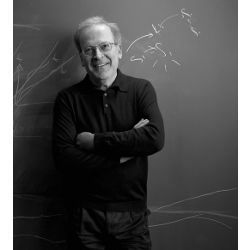
\includegraphics[scale=1.3]{LeslieValiantBW.png}
\captionof{figure}{Leslie Valiant}



\end{minipage}
\subsection{Aufbau einer BSP Maschine}
Um ein BSP-System zu Implementieren werden zunächst einige Dinge benötigt, zum einem handelt es sich um einen MIMD Ansatz, Multiple Instruction Multiple Data, also benötigt man mehrere Prozessoren die jeweils einen dedizierten Speicher haben.[1]\\
Im BSP wird auch eine Kommunikation zwischen den Prozessoren, oft in einem Netzwerk, benötigt. Wie man dieses Netzwerk gestaltet liegt zunächst in der Hand des Systemerstellers. Um eine Datenübertragung zwischen den Prozessoren zu gewährleisten, müssen die Verbindungen über einen Router laufen der dafür sorgt, dass die Prozessoren sich untereinander Daten versenden können. Die Kommunikation ist getrennt von jeglicher Synchronisation. Die Synchronisation ist Teil der Barriere welche garantiert, dass der Datenaustausch zwischen allen Prozessoren abgeschlossen ist. Mit dem Abschluss der Kommunikation werden die übertragenen Daten für den einzelnen Prozessor zugänglich, die sogenannte "Barrier-Synchronisation". Demzufolge arbeiten alle Prozessoren erst dann weiter, wenn der Datenaustausch und die Synchronisation abgeschlossen sind[1].

\newpage

\section{BSP Algorithmen}
Wie man schon aus dem Aufbau einer BSP Maschine erkennen kann, besteht auch der Algorithmus eines BSP Programms aus drei Teilen. Wie in Abbildung 2 gezeigt, wird zuerst die Rechenarbeit die jedem Prozessor zugeteilt wurde abgearbeitet, dann beginnen die Prozessoren untereinander Daten zu verschicken und im letzten Schritt werden diese Daten dann lokal für die einzelnen Prozessoren sichtbar. Diesen Ablauf nennt man einen \textit{Superstep}.\\
Ein BSP-Algorithmus besteht aus einem oder mehreren Supersteps. In einem Superstep werden möglichst viele Aktionen bzw. Befehle untergebracht, damit man alle verteilten Prozessoren möglichst gut auslasten kann, daher stammt auch der Begriff "Bulk" zu deutsch "Masse oder auch großes Bündel".  	


\begin{figure}[h]
	\centering 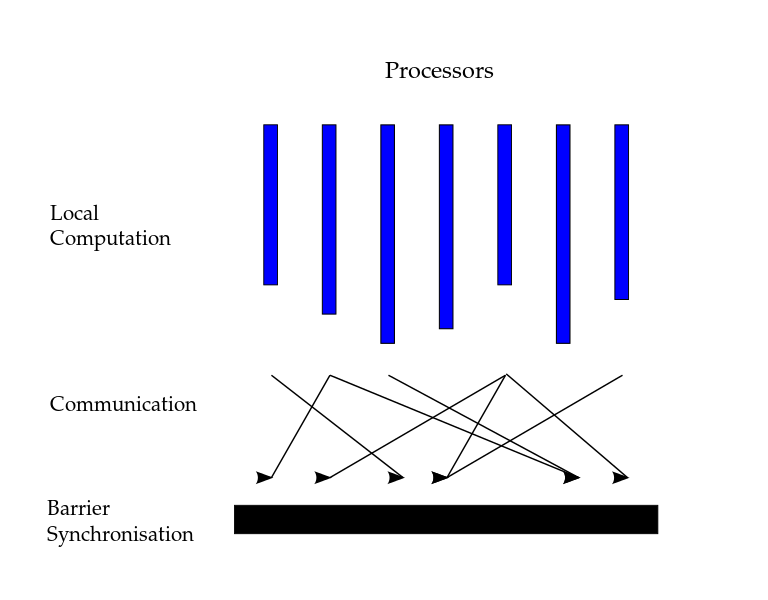
\includegraphics[scale = 0.4]{superstep.png}
	
	\caption{Ein Superstep}
\end{figure}



\subsection{Kommunikation}
Die Kommunikation in einem BSP-System ist nicht ganz mit der Kommunikation in einem verteilten System zu vergleichen. Wo in einer Kommunikation über ein Netzwerk eher ein \textit{send} und \textit{recieve} stattfindet, ist es in BSP eher mit einem Speicherzugriff der Art \textit{remote direct memory access} zu vergleichen. Ein \textit{RDMA} ist ein direkter Zugriff, der Art \textit{put} und \textit{get}, auf den Speicher eines Computers über ein Netzwerk, ohne das ein Betriebssystem Aufruf stattfindet[11].\\
In BSP werden alle Nachrichten sofort und ohne Verzögerung versendet. So eine "Massenversendung" hat den Vorteil, dass man eine Obergrenze an Zeit festlegen kann, die eine Kommunikation benötigt und damit zur Berechenbarkeit beiträgt. 

\subsection{Barriere}
Der Schritt weg von einer einheitlichen Kommunikation und Synchronisation, zur Auftrennung dieser beiden in Kommunikation und Barrierensychronisation, wirkt auf den ersten Blick aufwändig und kompliziert. Bei näherer Betrachtung der Nachteile die ein einheitlicher Datenaustausch mit der Datenverarbeitung mitbringt, kommt man schnell auf das Problem \textit{Deadlock} oder einer anderen Form den \textit{Livelock}, eine Verklemmung durch Abhängigkeiten der Prozessoren untereinander die dazu führt, dass nicht mehr weiter gerechnet werden kann. In BSP geht man diesem Problem der Verklemmung komplett aus dem Weg, eben weil eine Barriere keine ringförmigen Abhängigkeiten zwischen Daten kreieren kann[4].\\
Die Optimierung der Barriere ist in einem BSP-System essentiell da, an einer gut implementierten Barriere die Performance des Systems steht oder fällt. Die StandardBSPlib benutzt als simplen Optimierungsschritt einen Overhead, bei der Übertragung von Datenpaketen, welcher eine Information über die Größe des versendeten Paketes gibt. Solch ein Ansatz erhöht den benötigten Speicher und die Größe der Nachricht nur minimal, erhöht aber das Potential für Optimierungen enorm. Jeder Prozessor weiß nun wie groß die Pakete sind die er Empfangen wird. Das macht es einfacher Einstellungen bei der Programmierung der Barriere zu setzen[1].

\subsection{Kosten}
Die allgemeinen Laufzeitkosten in einem Superstep werden bestimmt von drei Faktoren: Kosten des am längsten zu rechnenden Prozesses, den Kosten des Datenaustausches zwischen den Prozessoren und die Kosten für die Barrierensynchronisation und das Beenden des Supersteps.\\

Die Kosten eines Supersteps für \begin{math}\mathcal{P} \end{math} Prozessoren:\\
\[\mbox{\textit{Superstep} = }\max_{i=1}^P (w_i) + \max_{i=1}^P (h_i g) + l\] 
$w_i$ sind die Kosten für die lokale Berechnung in dem Prozess $i$, und $h_ig$ beschreibt, die Anzahl der Nachrichten die ausgetauscht wurden von Prozess $i$, wobei $g$ die Permeabilität, also die Durchlässigkeit des Netzwerks bei hoher Last beschreibt, ein niedriger Wert für $g$ ist besser. Es wurde angenommen, dass die Prozesse alle gleichwertig sind. Eine häufige Form der Formel steht oft so in den Büchern $w + hg + l$, wobei $w$,$l$ Maximumsfunktionen sind.\\
Die Gesamtkosten eines BSP Algorithmus sind wie folgt beschrieben:\\
\[W + Hg + Sl = \sum\limits_{s=1}^S w_s + g \sum\limits_{s=1}^S h_s + Sl \]
$S$ ist die Anzahl der Supersteps. $W$, $H$, $S$ sind oft als Funktionen definiert die je nach Problem variieren können[1][4]. 


\newpage

\subsection{Code Beispiel}
Im Folgenden wird an einem Code Beispiel der Ablauf eines BSP Algorithmus deutlich erklärt. Verwendet wurde dabei eine Bibliothek von Albert-Jan N. Yzelman, welche er in seiner Promotion entwickelte und auch später weiter führte. Die entwickelte Bibliothek MulticoreBSP für Java und C, ermöglicht es auf modernen Mehrkernprozessoren ein BSP System zu implementieren[7].\\\\
Hier wurde ein simpler Ansatz gewählt, um die Vorgehensweise zu verdeutlichen. Es wird in einem Superstep über zwei Prozessoren zunächst die Oberfläche und das Volumen einer gegebenen Kugel berechnet. Nach diesem Superstep wird eine Barrierensynchronisation durchgeführt und der erste Prozessor berechnet, mit den synchronisierten Daten, dann im zweiten Superstep wie oft diese Kugel in einen Kubikmeter passen. Der Code wurde für eine vier Prozessor CPU implementiert. Im folgenden nehmen wir an das ein Thread für eine CPU steht.\\
\begin{lstlisting}
#define _PI 3.14159265358979323846 /*pi*/
#define circumference 10.0f
static double rad = circumference / (2 * _PI);
   
\end{lstlisting}
Zuerst werden benötigte Variablen global in C definiert, PI und der Durchmesser der Kugel. Alle Threads können nun darauf zugreifen. Globale Daten stellen die Vorbedingung für den Superstep dar, die durch vorangegangene Supersteps gesetzt wurden oder bei der Initialisierung erstellt werden.

\begin{lstlisting}
    double a = 0.0;
    
    bsp_begin(1);//Creates Thread 0  
    //Registers memory location for communication  
    bsp_push_reg(&a, sizeof(double));   
    bsp_init(&spmd2_entry, 0, NULL);//prepares Entrypoint for spmd2    
\end{lstlisting}
Variable \texttt{a} wird für den Superstep als neue globale Variable registriert, worauf dann auch eine Barrierensynchronisation stattfindet. Es wird dann \texttt{Thread 0}  erstellt, dieser ermöglicht nun den ersten Superstep einzuleiten.

\begin{lstlisting}
void spmd2_entry(void)
{    
    bsp_begin(2); //Generate 2 Threads
    double local = 0.0f;//local memory
    if(bsp_pid() == 1)//Thread 1 Calculates the Sphere volume
    {       
        local = (4/3) * _PI * (rad*rad*rad);
        bsp_push_reg(&local, sizeof (double) ); // Registers memory location for communication
    }    
    else //Calculates Area
    {   local = 4 * _PI * (rad * rad);
        bsp_push_reg(&local, sizeof (double) );
    }    
    bsp_sync();//signals the end of a Superstep and starts global communication
    bsp_end();//ends the called thread by bsp_begin()
} 

\end{lstlisting}
Nachdem im \texttt{Thread 0} der Superstep eingeleitet wird, beginnt zuerst die lokale Berechnung der einzelnen Threads hier rechnen zwei Threads parallel. Beide Threads haben einen lokalen Speicher \texttt{local}. \texttt{Thread 1} berechnet das Volumen der Kugel und \texttt{Thread 2} die Fläche. Mit \texttt{bsp\_sync} wird dann die Barrierensynchronisation eingeleitet. 

\newpage

\begin{lstlisting}
void spmd2_p0(double * const a)
{
 /*write Data of Threads in array*/
    for(unsigned int s = 0; s < bsp_nprocs(); ++s)
    {
        bsp_direct_get(s,array,0,array + s, sizeof(double));
        
        printf("Thread %d has result: %lf\n", s, array[s]);
        
       *(a+s-1) = array [s]; 
   }
    
    free(array);
}
\end{lstlisting}
Beide Threads übergeben nun ihre lokalen Daten an die Barriere, die in \texttt{spmd2\_p0} definiert ist. Hier wurde dies durch ein n-Thread großes Array gelöst, \texttt{Thread 0} schreibt in Element 0, \texttt{Thread 1} in Element 1 und so weiter.\\
In der Anfangs definierten Globalen Variable a wird nun der Feldeintrag geschrieben der für die weitere Berechnung erforderlich ist.

\begin{lstlisting}
void spmd1(void){
	if(bsp_pid() == 0){
    
	    printf("\nThread 0 calculates how many spheres will fit in an cubic 1 m cube...\n");                 
        bsp_direct_get(0, &a, 0, &volumeSphere, sizeof(double));}//get data from thread 1     
    
        /*cubic 1m = 1 000 000 cubic cm under the assumption the spheres will fill approx. 60% of the given space there is a volume of 600 000 cubic cm to fill*/
        /*Thread 0 calculates how many Spheres will fit in a cubic 1m square*/
        int volumeFit = 600000 / volumeSphere;
        printf("cubic 1m will be filled approx. by %d spheres with %.4f cm circumference.\n", volumeFit, circumference);
    
    bsp_end();
}
\end{lstlisting}
Zurück in \texttt{Thread 0} wird nun die globale Variable \texttt{a} mit den errechneten Werten aus dem vorhergehenden Superstep in einem neuen, dem	 zweiten,  verwendet um zu berechnen wie viele dieser Kugeln mit dem berechneten Volumen in einen Kubikmeter Würfel passen. Als letzten Schritt wird errechnete Anzahl noch auf dem Bildschirm ausgegeben und der zweite Superstep kommt zu einem Ende.	\\ 

Es wurden alle Aspekte eines BSP Algorithmus gezeigt, zuerst wurden die globalen Daten definiert, mit denen die Prozessoren rechnen. Danach wurde der erste Superstep eingeleitet, der mit einer unabhängigen Berechnung der zwei Prozessoren begann. Mit dem Ende der Berechnungen leitet man eine Kommunikation ein, die versendeten Daten beider Prozessoren werden in der Barriere in einem Array gespeichert und dann für den nächsten Superstep freigegeben. Es folgte der zweite Superstep, der exakt gleich Ablief, aber zum Ende hin keine Kommunikation benötigte also wurde der Superstep nach der Rechenzeit beendet und das Programm terminiert.
\newpage

\section{Optimierung}
Ein Programmierer ist immer dazu angehalten die Laufzeit eines Systems, und Codes, so klein wie möglich zu halten. Unter der BSPlib gibt es auch einige Ansätze der Optimierung, so wird das Programm eher kaum in den Fokus einer Optimierung gesetzt. Der Großteil der Optimierung findet in der abstrakten BSP Maschine statt und da vor allem in der Kommunikation zwischen den Prozessoren. Im Folgenden werden einige implementierte Verbesserungen der BSPlib vorgestellt.

\subsection{Message Packing}
Um die Netzwerklast zu minimieren, packt man bei Message Packing mehrere Pakete, die an zwischen zwei Netzwerkteilnehmern verschickt werden, zu einem zusammen. Das Kostenmodell von BSP fordert, dass eine Nachricht von z.B., 500-Byte genauso viel Speicher und Zeit kosten soll, wie 500 1-Byte große Nachrichten. Um diesen Grundsatz zu erfüllen, setzt man in der BSPlib Message Packing ein, demzufolge wird der Overhead einmal pro Prozessorpaar beansprucht und nicht bei jeder Nachricht erstellt[1].

\subsection{Destination Scheduling}
Wie vorher erklärt treten die Prozessoren alle gleichzeitig in die Kommunikation über, also wenn ein Prozessor anfängt Daten zu versenden werden die anderen eben so ihre Daten losschicken. Angenommen alle Prozessoren wollen als ersten Kommunikationsschritt etwas an Prozessor 1 schicken, so ist dieser Prozessor sichtlich schnell überlastet und das Netzwerk fällt in einen Busy-Wait. So ein Vorgehen ist in SPMD (Single Process Multiple Data) Programmiermodellen oft der Fall und führt daher auch zu Problemen. Die BSPlib geht mit solche Massen von Anfragen zu einem Prozessor hin anders um. Zum einen ist die Reihenfolge wie Nachrichten versandt werden nicht festgelegt, sie wird zufällig bestimmt[1]. Dadurch ist die Wahrscheinlichkeit einer auftretenden Massenkollision nahezu gebannt und wirkt sich sehr positiv auf die Performance aus.
\subsection{Pacing}
Ein Netzwerk besteht aus vielen Komponenten, oft behindern sich einige gegenseitig und Formen einen Engpass, oder auch Bottleneck. Ein Bottleneck kann bis zu einer bestimmten Höhe an Transaktionen vollkommen ohne Auswirkungen für ein System sein, nur mit ansteigender Transaktionsrate in dem Netzwerk, steigt auch die Gefahr, dass ein Bottleneck Einfluss auf die Performance nimmt, oder sogar zu einem Totalausfall führen kann. Um so etwas vorzubeugen, benutzt man Pacing. Pacing ist eine Drosselung des Systems, kurz unterhalb der maximal möglichen Übertragungsrate in diesem System. So ist gewährleistet, dass das System nicht in eine Situation kommt auszufallen, es ist im schlimmsten Fall langsam[1].
\newpage
\section{BSP in der Softwareentwicklung}
Mit der steigenden Nachfrage von Parallelensystemen werden viele verschiedene Lösungen auf dem Markt angeboten. Eine beliebte Lösung ist heutzutage in Form von Computerclustern zu finden. Ein Cluster, ist im eigentlichen Sinne ein Zusammenschluss vieler Rechnereinheiten, also sozusagen über eine Netzwerk verbundene Computer. Cluster sind modular aufgebaut und bieten die einfache Möglichkeit, Komponenten hinzuzufügen oder auch zu entfernen. \\
Ein Cluster eignet sich gut um, ein BSP-System aufzusetzen. In der Praxis gibt es mehrere Beispielsysteme: Apache Giraph, molekular dynamische Simulationen und Simulationen für Elektromagnetische Felder. Die zuletzt genannten sind in der Forschung sehr hilfreich und aussagekräftig, mit BSP lassen sich solch Mathematisch aufwändigen Prozesse in einer akzeptablen Zeit Simulieren und Auswerten. Apache Giraph ist ein Graph Analyse System[8] welches eine große Flexibilität und Skalierbarkeit bietet. Das auf Java aufgesetzte Framework, profitiert von der steigenden Nachfrage von sogenannten Big Data Analytics, also sehr große Datenmengen die man nicht mehr mit konventionellen Methoden der Analyse beherrschen kann, dafür ist die Menge an Daten zu schnell lebig. Facebook hatte im Jahr 2012 einen Datendurchsatz von 200TB pro Stunde[9]. Seit 2013 setzt Facebook, das BSP System Apache Giraph ein, um diese Daten Mengen zu Analysieren und Greifbar zu machen. Mit den gewonnenen Erkenntnissen werden die Suchfunktionen, und die Werbeschaltungen für den individuellen Nutzer optimiert[10].
\section{Zusammenfassung}
Bulk-Synchrounus-Parallel ist als Idee von einer neuen Herangehensweise an Programmiermodelle in Parallelensystemen gestartet und ist heute nicht nur ein theoretisches Modell sondern, auch ein etabliertes System in der Verarbeitung von großen Datenaufkommen. BSP kann die Antwort darauf bieten wie, man mit dem neue aufkommendem Thema Big Data umgeht. Apache liefert mit Giraph schon die erste Antwort darauf. Als Erkenntnis kann man sagen, BSP erfüllt alle notwendigen Bedingungen eines Programmiermodelles, aber macht auch einige Dinge anders als in den 1990er Jahren etablierte Modelle.\\
Der Aufbau einer BSP Maschine etabliert schon einen ersten Unterschied zu geläufigen Systemen, es wird die Definition einer Barriere gefordert. Weitere Anforderungen sind nur ein Netzwerk und die entsprechenden Recheneinheiten, so wie bei anderen verteilten Systemen auch. Festellen kann man hier, das die Definition einer Barriere der größte Aufwand bei dem Erstellen einer BSP Maschine darstellt.\\
In dem Aufbau eines BSP Algorithmus, zeigt sich recht schnell, dass keine direkte Herangehensweise geführt wird. Besonders in der Kommunikation zwischen den Prozessoren zeigt sich, dass es nicht immer die beste Wahl ist Daten sofort zu verschicken. Ein direktes Versenden ist natürlich, schneller als die in BSP etablierte Methode, dennoch müssen bei dem direkt Versand andere Probleme wie Deadlock, Livelock gelöst werden, welche die Performanz wieder drosseln. Daraus folgt: Einen geordneten Kommunikationsablauf zu vollziehen übergeht, im Gegensatz zu ungeordneten Abläufen, so manche Probleme und eröffnet neue Möglichkeiten für Optimierungen und Performanz. Im Gegenzug dazu hat eine direkte Versendung von Daten auch einen Vorteil, die Prozessoren müssen nicht wie auf Abb.1 gut zu sehen, auf den Start der Kommunikation warten, sie können direkt versenden.\\  
Es zeigt sich auch die Flexibilität und Einfachheit des BSPlib Standards, in dem es Projekte gibt ein BSP System auf einem Mehrkernprozessor auszuführen. Inwieweit dies Praktikabel ist, sei dahingestellt, aber es gibt in Zukunft sicher auch neue Methoden und Bestrebungen die Performance von Multicore Prozessoren zu optimieren. Eventuell findet man für Multicore sowie für parallele verteilte Systeme im theoretischen Modell BSP, eine Basis zur Entwicklung eines Highlevel Programmiermodells.\\




\newpage
\section{Referenzen}
\begin{enumerate}[label={[\arabic*]}]


\item R.Correa et al (eds), Models for Parallel and Dirstibuted Computation. Theory, Algorithmic Techniques and Applications S.: 85-115

\item Michael J Flynn IEEE Transactions on Computers. Vol. c-21, No.9, September 1972 \url{http://www.cs.utah.edu/~kirby/classes/cs6230/Flynn.pdf} (Abruf 01.01.2017)

\item Leslie G. Valiant, A bridging model for parallel computation, Communications of the ACM, Volume 33 Issue 8, Aug. 1990 

\item Paul Tarau PARALLEL PROCESSING AND ALGORITHMS, Fall 2014
\url{http://www.cse.unt.edu/~tarau/teaching/parpro/papers/Bulk%20synchronous%20parallel.pdf} (Abruf 01.01.2017)
\item University of Oxford Parallel Applications Centre
\url{http://www.bsp-worldwide.org/implmnts/oxtool/}(Abruf 01.11.2016)
\item Klaus-Dieter Krannich TU-Cottbus Paralleles Rechnen
\url{https://www.math.tu-cottbus.de/~kd/parallel/vorl/vorl/node18.html}(Abruf 11.11.2016)
\item Universität Utrecht Albert-Jan Yzelman, Rob Bisseling
\url{www.multicorebsp.com}(Abruf 01.01.2016)
\item \url{http://giraph.apache.org/apidocs/}
\item Buyya, Rajkumar, Rodrigo N. Calheiros, and Amir Vahid Dastjerdi. Big Data: Principles and Paradigms.Cambridge, MA, USA: Morgan Kaufmann is an imprint of Elsevier, (2016):
\item Joab Jackson  PC World Korrespondent
\url{http://www.pcworld.com/article/2046680/facebooks-graph-search-puts-apache-giraph-on-the-map.html}(Abruf 01.02.2017)
\item A Critique of RDMA By Patrick Geoffray, Ph.D. August 18, 2006
\url{https://www.hpcwire.com/2006/08/18/a_critique_of_rdma-1/}(Abruf 20.01.2017)
\end{enumerate}
\section{Abbildungen}
\begin{itemize}
\item Abbildung 1 \url{http://cacm.acm.org/magazines/2011/6/108643-beauty-and-elegance/fulltext}
\item Abbildung 2 \url{https://upload.wikimedia.org/wikipedia/en/thumb/e/ee/Bsp.wiki.fig1.svg/768px-Bsp.wiki.fig1.svg.png}
       
\end{itemize}





\end{document}
